\section{Results}
\label{c6:sec:results}

\subsection{Baseline characteristics}
The mean age of the patients was 66.7 years, and 71.9\% were men (Table~\ref{c6:table:1}). Most patients were in NYHA class I or II (73.8\%). The median baseline NT-proBNP value was 137.3 pmol/L (IQR: 51.7-272.6). A total of 2022 NT-proBNP measurements were performed during follow-up before the PE occurred. The PE occurred in 70 patients (26.6\%). The median maximum follow-up time was 2.1~(IQR: 1.2--2.4) years.

\begin{table}
\small
\centering
\caption{\textbf{Summary of the Bio-SHiFT dataset}. The primary study endpoint (PE) was defined as the composite of cardiac death, cardiac transplantation, left ventricular assist device implantation, or hospitalization for heart failure, whichever occurred first. Abbreviations: NYHA is New York Heart Association Classification~\citep{bredy2018new}; IQR is interquartile range.}
\label{c6:table:1}
\begin{tabular}{p{8cm}r}
\toprule
\textbf{Characteristic} & Value\\
\midrule
Total patients & 263\\
\emph{PE (primary endpoint)} & 70\\
\midrule
Total NT-proBNP measurements & 2022\\
Median NT-proBNP (pg/mL) & 110.3 (IQR: 38.5--240.9)\\
Median age at inclusion (years) & 67.9 (IQR: 58.9--75.8)\\
Median BMI at inclusion & 26.5 (IQR: 24.4--30.1)\\
Median NYHA (assumed continuous) & 2 (IQR: 1--3)\\
$\mbox{Gender} = \mbox{Female}$ (\%) & 74/263 (28.1\%)\\
$\mbox{Renal failure history} = \mbox{Yes}$ (\%) & 136/263 (51.7\%)\\
$\mbox{Type-II diabetes mellitus} = \mbox{Yes}$ (\%) & 81/263 (30.8\%)\\
\midrule
Median maximum follow-up per patient (years) & 2.1 (IQR: 1.2--2.4)\\
Median \#NT-proBNP per patient & 9 (IQR: 5--10)\\
\bottomrule
\end{tabular}
\end{table}

\subsection{Association between temporal patterns of NT-proBNP and the PE}
Serially measured NT-proBNP was associated with the PE (univariable HR per doubling of NT-proBNP:~2.13, 95\%CI:~1.81--2.53, p<0.001). After adjustment for age, gender, diabetes mellitus, NYHA class, body mass index, and renal function, serially measured NT-proBNP remained independently associated with the PE (adjusted HR per doubling of NT-proBNP:~2.20, 95\%CI~:1.84--2.68, p<0.001). Two examples of dynamic risk assessment of individual patients from the Bio-SHiFT dataset based on the joint model are demonstrated in Supplemental Materials, Figure 1A-B. 

\subsection{Fixed versus personalized screening schedule: high-risk interval and number of measurements}
The median follow-up time of the 750 patients in the simulated dataset was 1.76 years~(IQR:~1.42--2.24); mean~(standard deviation) was 1.85~(0.63) years and the maximum was~3.5 years. The personalized schedule used fewer measurements as compared to the fixed (Panel~A, Figure~\ref{c6:fig:2}). The personalized schedule used a median of 7~(IQR:~7--8) and the fixed schedule, a median of~9~(IQR:~8--10) measurements. Corresponding cost estimates are demonstrated in the Supplemental Materials. The start of the high-risk intervals for the fixed and personalized screening schedules are depicted in Figure 2B. The personalized and fixed schedules showed similar results, i.e., the difference between the estimated intervention time compared to the `true' event time was a median of~6.6~(IQR:~4.5--11.3) months for the personalized and a median of~6.3~(IQR:~4.2--10.3) months for the fixed schedule (Panel~B, Figure~\ref{c6:fig:2}). In both schedules, scheduling of new sampling moments was stopped in order to undertake appropriate action, well in time before the event occurred.

\begin{figure}
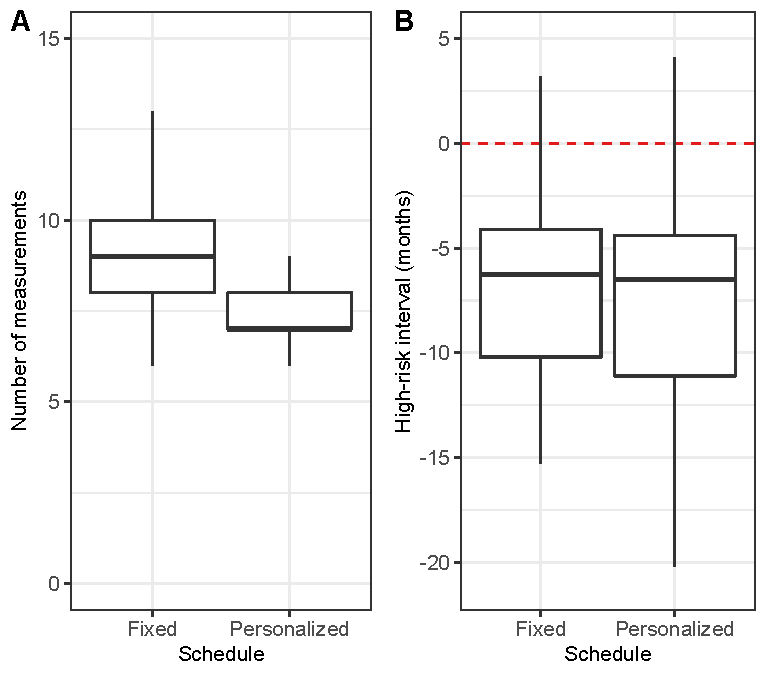
\includegraphics{contents/c6/images/c6_fig2.pdf}
\caption{\textbf{Total NT-proBNP measurements and high-risk interval (months) preceding the primary endpoint (PE)} for fixed (quarterly measurements) and personalized schedules. Results are based on a realistic simulation study of 263 test patients. NT-proBNP is measured as per personalized and fixed schedules, until a patient's cumulative-risk of obtaining PE in the subsequent three months is above 7.5\%. The boxplot for the number of measurements in Panel~A is made using data of all simulated patients. The boxplot for the high-risk interval (the difference between the time at which NT-proBNP measurements are stopped and the true simulated PE time) in Panel~B, is based on only those patients who observe PE. In Panel~B a zero high-risk interval (dashed red line) indicates that no time is available for intervention before occurrence of PE.}
\label{c6:fig:2}
\end{figure}

Results of the analyses using risk thresholds of consecutively 5\% and 10\% over three months are depicted in the Supplemental Materials, Figure~\ref{c6:fig:app1}, and Figure~\ref{c6:fig:app2}, respectively. Based on a risk threshold of 5\% over three months, the fixed and personalized screening schedules demonstrated similar results for the high-risk interval. However, again, the personalized screening schedule used fewer measurements as compared to the fixed screening schedule. The same was true for the risk threshold of 10\%. In case of a risk threshold of 5\% over three months, we found that the start of the high-risk interval was further away from the true event time as compared to a risk threshold of 7.5\% over three months. Conversely, in case of a risk threshold of 10\% over three months, the start of the high-risk interval was closer to the true event time as compared to a risk threshold of 7.5\% over three months. These results comply with the increase in the risk threshold.